The mobile application layer has four subsystems, there is a subsystem for scheduling which allows the mobile app to create a set schedule for automation of the change of shutter positions. This allows a user to set a predefined time they want to change the shutters position and the shutters would automatically change positions without interaction from the mobile app. There is also a subsystem that defines how the shutters and the mobile app will communicate with each other

\subsection{Mobile Device Communications}
Mobile devices use the mobile application to send request to the hub.

\begin{figure}[h!]
	\centering
 	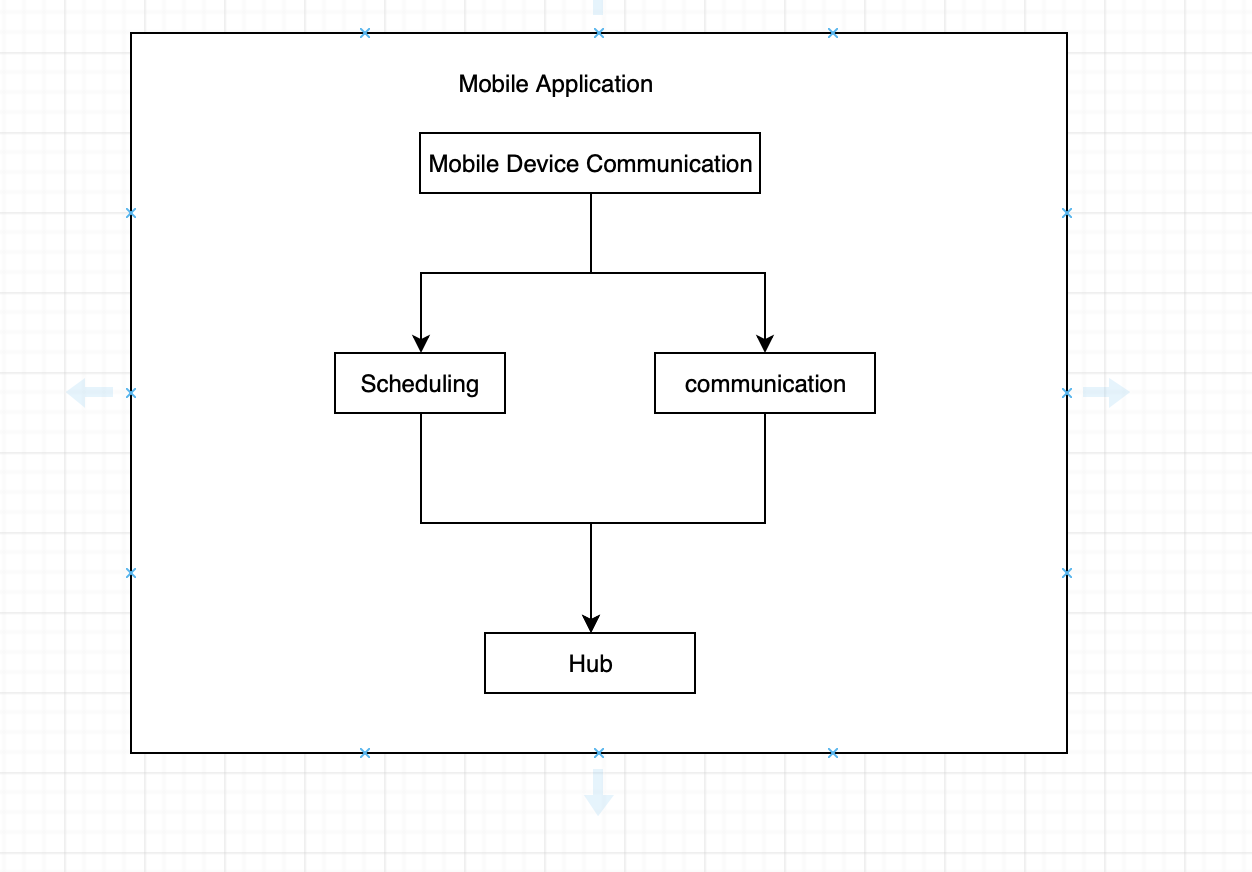
\includegraphics[width=0.60\textwidth]{images/Mobile}
 \caption{Example subsystem description diagram}
\end{figure}

\subsubsection{Assumptions}
Users have an android or ios phone and users have not tampered with the application. 

\subsubsection{Responsibilities}
Properly taking commands from the user and displaying all the option for the user as well as displaying the status of each shutter that is connected to the hub.

\subsubsection{Subsystem Interfaces}

\begin {table}[H]
\caption {Subsystem interfaces} 
\begin{center}
    \begin{tabular}{ | p{1cm} | p{7cm} | p{4cm} | p{5cm} |}
    \hline
    ID & Description & Inputs & Outputs \\ \hline
    1 &Allows users to choose between a scheduled or immediate task& Mobile device communication & scheduling and communication \\ \hline
    \end{tabular}
\end{center}
\end{table}

\subsection{Scheduling}
\subsubsection{Assumptions}
Users have an android or ios phone and users have not tampered with the application. 

\subsubsection{Responsibilities}
Properly executing tasks at the requested time.

\subsubsection{Subsystem Interfaces}

\begin {table}[H]
\caption {Subsystem interfaces} 
\begin{center}
    \begin{tabular}{ | p{1cm} | p{7cm} | p{4cm} | p{3cm} |}
    \hline
    ID & Description & Inputs & Outputs \\ \hline
    1 &Package all request and send to the hub&Scheduling &Hub\\ \hline
    \end{tabular}
\end{center}
\end{table}

\subsection{Communication}
\subsubsection{Assumptions}
Users have an android or ios phone and users have not tampered with the application. 

\subsubsection{Responsibilities}
Properly executing tasks at the requested time.

\subsubsection{Subsystem Interfaces}

\begin {table}[H]
\caption {Subsystem interfaces} 
\begin{center}
    \begin{tabular}{ | p{1cm} | p{7cm} | p{4cm} | p{3cm} |}
    \hline
    ID & Description & Inputs & Outputs \\ \hline
    1 &Package all request and send to the hub& Communications &Hub\\ \hline
    \end{tabular}
\end{center}
\end{table}

\subsection{Hub}
\subsubsection{Assumptions}
Users have an android or ios phone and users have not tampered with the application. 

\subsubsection{Responsibilities}
Properly executing tasks at the requested time.

\subsubsection{Subsystem Interfaces}

\begin {table}[H]
\caption {Subsystem interfaces} 
\begin{center}
    \begin{tabular}{ | p{1cm} | p{7cm} | p{5cm} | p{4cm} |}
    \hline
    ID & Description & Inputs & Outputs \\ \hline
    1 &Send all request to the Hub or the Shutters directly &Communications or Scheduling &WiFi or Bluetooth communication\\ \hline
    \end{tabular}
\end{center}
\end{table}
